\documentclass{article}
\usepackage{float}
\usepackage{amsmath}
\usepackage{graphicx}
\usepackage{geometry}
\usepackage{fontspec}
\usepackage[fontsize=12pt]{fontsize}
\usepackage[all]{xy}
\usepackage{booktabs}
\usepackage{listings}
\usepackage{tabularx}
\usepackage{enumitem}
\usepackage{fancyhdr}
\usepackage{caption}
\usepackage{indentfirst}

\numberwithin{equation}{section}
\geometry{a4paper,centering,scale=0.8}
% \setmainfont{Times New Roman}
% \setmonofont{Courier New}
\linespread{1.2}
\bibliographystyle{plain}
\lstset{%
	basicstyle=\rmfamily,
	keywordstyle=\bfseries,
	commentstyle=\itshape,
	columns=fullflexible,
	breaklines,
	tabsize=4}

\setlength{\belowcaptionskip}{9pt}
\setlength{\abovecaptionskip}{9pt}
\setlength{\headsep}{0.4in}
\setlength{\headheight}{14.5pt}
\captionsetup{font={footnotesize}}
\renewcommand{\baselinestretch}{1.0}
\geometry{bottom=1in}

\newcommand{\A}{Merchant $A$}
\newcommand{\B}{Merchant $B$}
\newcommand{\X}[1]{Merchant $#1$}
\newcommand{\RP}[1]{$RP_#1$}
\newcommand{\RPd}{$RP$}
\newcommand{\itembf}[1]{\item \textbf{#1}}
\newcommand{\itemsl}[1]{\item \textsl{#1}}
\newcommand{\tabincell}[2]{\begin{tabular}{@{}#1@{}}#2\end{tabular}}

\newcommand{\Problem}{E}
\newcommand{\Team}{22454775}
\newcommand{\wholepages}{25}
\title{\huge\textbf{Grand Title}}
\author{IMMC\#\Team}
\date{\today}

\pagestyle{fancy}
\fancyhead[L]{IMMC\#\Team}
\fancyhead[R]{Page \thepage \ of \wholepages}
\fancyfoot{}

\begin{document}
	\thispagestyle{empty}
\vspace*{-16ex}
\begin{center}
\centerline{\begin{tabular}{p{\linewidth}<{\centering}}
  \small Team Control Number \\
  \huge \textbf{\Team} \\
  \small Problem Chosen \\
  \huge \textbf{\Problem} \\
  \textbf{2022} \\
  \small \textbf{IMMC} \\
  \small \textbf{Summary Sheet} \\
  \hline
\end{tabular}}
\end{center}
	\hspace{\parindent} A loyalty points system is a decentralized platform based on blockchain, through which merchants can obtain benefits. By developing mathematical models, the influence of various factors on the yearly revenue of merchants in one-to-one alliances and many-to-many alliances are quantified and calculated, the way of distributing points optimized. The research on this problem provides suggestion and references for the future development of similar system and promote merchants to greater development.

In our first model, in order to determine the change in business yearly revenue for a merchant from a one-to-one alliance, we need to abstract the behavior of the alliance and find out the factors that affect the formation of alliance, so as to develop our model. Through programming, we develop the Revenue Change Model(1-1), and divide the customers into three groups by the merchants they have gone shopping for based on the data before and after joining the alliance. Then we calculate the benefit the alliance bring about to merchants. In addition, we calculate the losses from issuing \RPd s, and then calculate the annual growth rate of merchants based on these two results. By inputting the data, merchants can use the output to estimate their yearly revenue growth.

To measure the overall positive impact of a many-to-many alliance to an ally, we create the second model --- the Revenue Change Model (m-m). Through analysis, we find the key factors that affect the impact. By using data fitting and partial differential equations, we get the functional expression of the factors and conclude the expression to calculate the impact. The expressions can be found in the main text, which can determine the optimal number of merchants to form such an alliance with different business scales. Considering that different merchants bring different benefits to the alliance, we form a mathematical model and get a more reasonable way of allocating reward points. It is worth mentioning that in this model, we quantify the factors well and make it as close to the facts as possible, which makes the expression stricter.

We conduct a comprehensive sensitivity analysis on the model and analyze the arguments' influence on the model results. Most of the variables are proved to be insensitive, which shows that our model is reliable.

The highlights of this paper include: our Revenue Change Model(1-1) only depends on the data input by merchants, so it's rather independent, which means it's well-adapted and is easy to promote; at the same time, it can use data for a short period of time to estimate yearly revenue growth, so it's efficient. And our Revenue Change Model(m-m) is comprehensive. It covers many variables related to yearly revenue and is well quantified, which makes our expression stricter. In conclusion, we comprehensively analyze and determine the growth of yearly revenue after merchants join in one-to-one or many-to-many alliances, which has practical significance.
	\pagebreak
	\tableofcontents
	\thispagestyle{empty}
	\pagebreak
	
	\section{Introduction}
	\subsection{Background}
	Nowadays, the development of the Internet brings about the revolution of blockchain, which is a technology that stores, verifies, transfers and communicates network data through its own distributed nodes without relying on a third party.

So blockchain can be regarded as a community of network, which contributes to the merchants’ cooperation. With its decentralization, it can help build an open system, which is called the loyalty points system. Any merchant can join in, so that the reward points and interests of different platforms can be flexibly transferred and more benefits will be created.

Compared with general \RPd\ system, the loyalty points systems based on blockchain have advantages in many aspects, the first of which is its characteristic of decentralization, which wins customers' trust. While \RPd\ in a general \RPd\ system can be easily tampered, the loyalty points system is open and transparent,so the technology of blockchain can serve as an easy solution to the trust crisis.

Besides, unlike general \RPd\ systems which give out \RPd\ freely, the loyalty points system has a fixed model. This means that a loyalty points system usually has a fixed total number of \RPd\ (or the total number of \RPd\ is linearly related to some variable), which brings about more commercial value.

As \RPd s in the loyalty points systems own its independent commercial value and are value-added, such \RPd\ can be approximately regarded as tokens. Compared with general \RPd\ which can only be exchanged, \RPd\ in the loyalty points systems can even be used as equity.

Loyalty point system today is gradually becoming the main type of \RPd\ systems. As a system with so many advantages, it will definitely bring more energy and vitality to the marketplace in the future.
	\subsection{Problem Restatement}
	Under such a background, merchants can benefit themselves by joining in such a decentralized reward points system. Such a kind of system can be fallen into two forms: one-to-one alliance and many-to-many alliance.

We hope to build mathematical models to measure how benefits can be maximized in these two alliances. 

  \begin{itemize}  
  \item
  For the one-to-one alliance, we want to develop the factors that enable the alliance to obtain more benefits, then calculate its impact on the yearly revenue of merchants by our mathematical model.

  \item 
  For many-to-many alliances, we hope to find the suitable number of merchants in the alliances and the change of alliance pattern affected by yearly revenue and profit of each merchant.
  
  \end{itemize}  

In addition, as more and more merchants join in the many-to-many alliances, we want to give merchants different weights based on how much they contribute. To achieve this, we need to develop a mathematical model to determine the amount of reward points allocated to a particular merchant in this alliance.
	\subsection{Our Work}
	\begin{enumerate}
	\itembf{Create a model to calculate the change in business yearly revenue for a merchant in a one-to-one alliance:}
		
	\begin{enumerate}[label=(\alph*)]
	\item Abstract the behavior of a one-on-one alliance.
	\item Find the key factors that affect the operation.
	\item Write a program (One-to-One Alliance Revenue Estimation Algorithm).
	
	Our model needs the data of merchants before and after joining the alliance. Using these data, we divide the customers into three groups by the merchants they have gone shopping for before the form of the alliance. Then we calculate respectively the additional benefit brought by buying a specific type of product and the losses from issuing \RPd s. The model provides merchants with their revenue growth rate.
	\end{enumerate}

	\itembf{Create a model to measure the overall positive impact of a many-to-many alliance to an ally:}

	\begin{enumerate}[label=(\alph*)]
	\item List the factors that affect $I$ and list the expressions to calculate $I$, the factors including $I_A$, $I_D$, $\phi$ and $RC$.
	\item Use partial differential equations to get the functional expression of $RC$.
	\item Get the mathematical expression of $I_A$, finding that the key factors affecting it include $n$.
	\item Find out how $I_D$ and $\phi$ relate to the factors and get the the functional expression of it.
	\item Explore the relationship between product types of every two allies in a many-to-many alliance and its impact on the alliance efficiency.

	By applying to the final expression, we can calculate $I$. It measures the overall positive impact on the merchant, which is related to how well a many-to-many alliance is formed. And the optimal number of merchants to form such an alliance can also be calculated, it changes as $s$ changes, indicating that the optimal number of merchants varies to the allies.
	\end{enumerate}

	\itembf{Conduct sensitivity analyses of our model:}
		
	To assess the robustness of our model, we conduct sensitivity analyses on $n$, $\phi$ and $s$. From the final result, we discover that the change of yearly revenue of each merchant won't affect the alliance model.

	\itembf{Find the optimal distribution of \RPd :}
	Since different merchants in an alliance bring different benefits to the alliance, they should be allocated different amount of \RPd\ according to the conditions. What we need to do is to provide a more reasonable distribution for \RPd\ through modeling.

\end{enumerate}
	
	\section{Nomenclature}
	\begin{table}[H]
\begin{tabularx}{\textwidth}{cX}
	\toprule
	$RP_X$ & (the number of) Reward Point (from Merchant $X$) \\
	\midrule
	$RPU_{x,X}$ & the amount of \RPd\ used when purchasing Product $x$ in Merchant $X$ \\
	\midrule
	$s_X$ & the scale (market value) of an ally in an alliance \\
	\midrule
	$\overline{s}$ & the average scale of all allies in a many-to-many alliance \\
	\midrule
	$\theta_X$ & the yearly sells of \X{X} \\
	\midrule
	$I$ & the overall positive impact of a many-to-many alliance to an ally \\
	\midrule
	$RC$ & the community cover rate of all allies in a many-to-many alliance \\
	\midrule
	$n$ & the number of merchants in a many-to-many alliance (the branch stores count)\\
	\midrule
	$\Phi_{X}$ & the product type scale for \X{X}\\
	\midrule
	$\phi_{i,X}$ & the product type scale by \X{X} by products in Product Type $i$ \\
	\midrule
	$M_\alpha$ & the max index (number) of Object $\alpha$ (product/product type/customer) \\
	\midrule
	$PT_x$ & the index of the Product Type of Product $x$ \\
	\midrule
	$P_x$ & the price of Product $x$ \\
	\midrule
	$k_1$ & the conversion rate from currency to \RPd \\
	\midrule
	$k_2$ & the conversion rate from \RPd\ to currency (discount) \\
	\midrule
	$T$ & the time span of data before the form of the alliance \\
	\midrule
	$L_c$ & the label of Customer $c$ \newline (-1 stands for not labeled, 0 stands for having only purchased from Merchant $A$, 1 stands for from Merchant $B$, 2 stands for from Merchant $A$ and $B$, all before the form of the alliance) \\
	\midrule
	$N_{x,X}$ & the number of times Product $x$ is purchased in \X{X} before the form of the alliance \\
	\midrule
	$E_{x,X,c}$ & the profit efficiency (amount of profit made per unit time) of Product $x$ from Customer $c$ in Merchant $X$ before the form of the alliance \\
	\midrule
	$R_{x,X}$ & the revenue of \X{X} by Product $x$ before the form of the alliance \\
	\midrule
	$\Delta_{x,X}$ & the rate of bonus revenue brought about by Product $x$ and by the alliance to \X{X} \\
	\midrule
	$T^\prime$ & the time span of data after the form of the alliance \\
	\midrule
	${N_{x,X}}^\prime$ & the number of times Product $x$ is purchased in \X{X} after the form of the alliance \\
	\midrule
	${R_X}^\prime$ & the revenue of \X{X} after the form of the alliance \\
	\bottomrule
\end{tabularx}
\caption{the nomenclature for 1-1 and m-m alliance}
\label{tab:nomenclature}

\phantom{shabi moxing}

The $x$, $i$, $c$ here means the index (of product or product type or customer).
\end{table}
	
	\section{Assumptions}
	\begin{enumerate}
	\item
	The market is a competitive market where the ultimate purpose of merchants is earning profits and that of customers is getting their needs at the lowest price.

	\item
	The relationship between used \RPd\ and the equal currency at the checkout is linear.
	
	\item
	If a customer goes shopping and has its reward points, the customer will choose to use it and obtain most discount.
	
	\textsl{
	This assumption is based on the last one. Since the relationship is linear, customers don't need to take into account how to spend the reward points reasonably to obtain most discount, and nor do we.
	}
	
\end{enumerate}
	
	\section{One-to-One Alliance}
	\subsection{Mechanism}
	In the first part we need to explain how the one-to-one alliance works and benefits the merchants.

\begin{figure}[H]
	\centering
	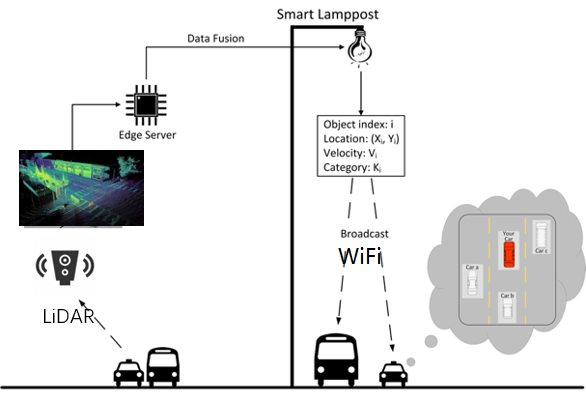
\includegraphics[width=\linewidth]{mechanism.png}
	\caption{the mechanism of the alliance}
	\label{fig:mechanism}
\end{figure}

Figure \ref{fig:mechanism} shows how the alliance system works. Suppose $x$ customers come to \A, do the purchase and obtain \RP{A}. Then they have needs for other products that \A\ does not offer. Since they can get a discount, a part of them will tend to go to \B. There they do the purchase, repeat the process and then return to \A. In the cycle, the number of the left customer is declining. As the customers return to the original merchant, the cycle comes to its end, which means the end of this round of benefit from \A\ to \B.
	\subsection{Factors}
	The essential requirement to form an alliance is that it can bring enough extra benefits. From Figure \ref{fig:mechanism}, we can know that the source of the extra benefits is the non-stopping needs of customers and the lure from the discounts brought about by the reward points.

Suppose the alliance (if formed) is formed by \A\ and \B.

\begin{enumerate}
	\itembf{Relative business size}
	
	If \A\ is famous while \B\ has no fame at all, customers will never purchase product from B and in turn get \RP{A}, or go to \B\ with the reward points from \RP{B}. Only when the allies bear similar fame will the alliance be formed.
	
	\itembf{Product type}
	
	Since the essential of the system is mutual advertisements, the allies should not block each other's business and maximize the stimulating effect of purchasing in its ally's store.
	
	\begin{enumerate}
		\itembf{Difference}
		
		As a business alliance, the allies should not block each other's business, meaning that the allies should not sell too same kinds of products.
		
		\itembf{Correlation}
		
		Since the essential of the system is mutual advertisements, the allies should maximize the stimulating effect of purchasing in its ally's store, so \A's products should mostly fit in the potential shopping list of \B's customers (and vice versa).
	\end{enumerate}
	
	\itembf{Distance between nearest offline stores}
	
	In the case of offline stores, since (suppose) the customers receive the recommendation (reward points) from \A, they would go back home and go for \B\ on another day, the nearest offline stores should be close enough for the customers to think the extra distance worth the discount.
\end{enumerate}



	\subsection{Revenue Change Model (1-1)}
	We use some basic data (both before and after the form of the alliance) from both merchants to show the percentage of the estimated benefit growth brought about by the alliance. The result (revenue growth) is specified to each type of product \textsl{(e.g. food, daily necessities etc.)}. Referencing the results, the merchant can adjust its stocking or "money-to-RP" ("RP-to-money") rates over time to reach the highest benefit. Also, after a short period of data collection, the merchant will be able to estimate the total benefit growth in one year. The process is explained below.
\newline

\begin{enumerate}[label=(\arabic*)]
\itembf{Profit Efficiency Calculation}

We estimate the amount of benefit made per unit time ($E$) to see how much benefit will the customers bring to the merchants after the form of the alliance, which still exists without the alliance. The benefit growth is estimated as:
\[  E_{x,X,c} = \frac{P_x \cdot N_{x,X}}{T}  \]

\itembf{Customer Classification}

We classify the customers into three classes according to the merchant they have made purchases in.

\begin{enumerate}[label=(\alph*)]
\item A.

These are customers who have only done purchases from Merchant A before the form of the alliance. They bring additional benefit buying a specific product type to Merchant B as:
\[
\sum\limits_{L_c  = 0} {\sum\limits_{x = 0}^{M_x} {\sum\limits_{c = 0}^{M_c } {N_{x,1,c}  \cdot P_x } } } \]

\item B.

These are customers who have only done purchases from Merchant B before the form of the alliance. They bring additional benefit buying a specific product type to Merchant A as:
\[
\sum\limits_{L_c  = 1} {\sum\limits_{x = 0}^{M_x}} {\sum\limits_{c = 0}^{M_c} } {N_{x,0,c}  \cdot P_x }
\]

\item A \&\ B.

These are customers who have done purchases from both Merchants. They bring benefit to \X{X} as:
\[
\sum\limits_{L_c  = 2} {\sum\limits_{x = 0}^{M_x} {\sum\limits_{c = 0}^{M_c} {N_{x,X,c}  \cdot P_x } } } \]

But they should provide the benefit for \X{X} after the form of the alliance as:
\[
\sum\limits_{L_c  = 2} {\sum\limits_{x = 0}^{M_x} {\sum\limits_{c = 0}^{M_c} {E_{x,X,c}  \cdot T'} } } 
\]

So they bring Merchant X an additional benefit of:
\[
\sum\limits_{L_c  = 2} {\sum\limits_{x = 0}^{M_x} } {\sum\limits_{c = 0}^{M_c} } {X_{x,X,c}  \cdot P_x  - E_{x,X,c}  \cdot T'} 
\]

In total, customers buying a specific type of product bring an additional benefit of:

\phantom{LATEX WO RI NI MA}

\noindent To A:
\[
\sum\limits_{L_c  = 1,2} {\sum\limits_{x = 0}^{M_x} } {\sum\limits_{c = 0}^{M_c} } {N_{x,0,c}  \cdot P_x }  - \sum\limits_{L_c  = 2} {\sum\limits_{x = 0}^{M_x} } {\sum\limits_{c = 0}^{M_c} } {E_{x,0,c}  \cdot T'}
\]

\phantom{LATEX CHAO JI SHA BI}

\noindent To B:
\[
\sum\limits_{L_c  = 0,2} {\sum\limits_{x = 0}^{M_x} } {\sum\limits_{c = 0}^{M_c} } {N_{x,1,c}  \cdot P_x }  - \sum\limits_{L_c  = 2} {\sum\limits_{x = 0}^{M_x}} {\sum\limits_{c = 0}^{M_c} } {E_{x,1,c}  \cdot T'}
\]

\end{enumerate}

\itembf{Losses from issuing RPs}

Merchants lose amount of benefit due to their distribution of \RPd. They are calculated here. Loss for Merchant X:
\[  RPU_{x,X} \cdot k_2  \]

\itembf{Results}

By adding up additional benefits and losses, we get the total benefit the alliance brings about.

For \A:
\[
\Delta _{x,0}  = \sum\limits_{L_c  = 1,2} {\sum\limits_{c = 0}^{M_c} } {N_{x,0,c} }  \cdot P_x  - \sum\limits_{L_c  = 2} {\sum\limits_{c = 0}^{M_c} {E_{x,0,c}  \cdot T'} - RPU_{x,0}  \cdot k_2 }
\]

For \B:
\[
\Delta _{x,1}  = \sum\limits_{L_c  = 0,2} {\sum\limits_{c = 0}^{M_c} } {N_{x,1,c} }  \cdot P_x  - \sum\limits_{L_c  = 2} {\sum\limits_{c = 0}^{M_c} {E_{x,1,c}  \cdot T'} - RPU_{x,1}  \cdot k_2 }
\]

While the original benefit is:
\[  R_{x,X} = T^\prime \cdot \sum\limits_{c=0}^{M_c} E_{x,X,c}  \]

So the growth for Product Type $i$ and Merchant X will be:
\[
\frac{{\sum\limits_{PT_x  = i} {\sum\limits_{x = 0}^{M_x} {\Delta _{x,X} } } }}{{\sum\limits_{PT_x  = i} {\sum\limits_{x = 0}^{M_x} {R_{x,X} } } }} \cdot 100\% 
\]

While the total growth of Merchant X:
\[  \frac
{\sum\limits_{x=0}^{M_x} \Delta_{x,X}}
{\sum\limits_{x=0}^{M_x} R_{x,X}}
\cdot 100\%
\]

\end{enumerate}

We realize these features through programming. The program is in \textsl{Appendix A}.
	
	\section{Many-to-Many Alliance}
	\subsection{Factors}
	\begin{enumerate}
	\itembf{Business size}
	
	As written in 4.2, only when the allies bear similar fame will the alliance be formed. And it can also apply to many-to-many alliances partly. For a many-to-many alliance, only big businesses can afford the cost of \RPd\ and benefit each other. (If only one merchant is famous enough, then most of its customers will go to other merchants in the alliance while itself will get a few new customers.) So a many-to-many alliance can only contain big businesses.
	
	\itembf{Product type}
	
	As the essential of the alliance does not change when the number of merchants rise, the impact of product type is similar.
	
	\begin{enumerate}
		\itembf{Difference}
		
		If the allies sell too similar products, they may get involved in vicious competitions, leading to unwanted results.
		
		\itembf{Correlation}
		
		Due to the mutual advertisements effect of the system, allies should maximize the stimulating effect of purchasing in its ally's store, so each ally's products should mostly fit in the potential shopping list of the one of others'.
	\end{enumerate}
	
	\itembf{Size of the community}
	
	Each merchant owns its own group of customers, adding up to their community. When a merchant joins in an alliance, its own community will be added to the alliance community. So the more merchants the alliance contains, the more its community will be, which means there will be more customers. (It should be remembered that different merchants may have same customers.)

\end{enumerate}

	\subsection{Model Assumptions}
	\begin{enumerate}
\item
Every merchant has its impact on its neighboring 200 meters.

\textsl{
This is partly based on the reality --- on this condition, as the number of allies ($n$) rises, $RC$ increases and $\frac{d}{dn} RC$ decreases.
}

\item
In every given limited area, all customers are averagely distributed.

\textsl{
Under this circumstance, the relationship between $RC$\ and its impact is linear.
}

\item
All the allies in the alliance are listed companies.

\textsl{
We need to quantify the scale of every ally. We decide to measure it by the company's market value. 
}
\end{enumerate}
	\subsection{Revenue Change Model (m-m)}
	\subsubsection{General Route}
In this model, we estimate the overall positive impact of a many-to-many alliance to one ally.

When a customer does a purchase in an ally, he receives \RPd s for the alliance. Then he will browse where he can use them for a discount. This gives a chance of advertisement for every ally in the alliance.
But at the meantime, if an ally is not famous, when a customer views the list of allies in the alliance, the customer may ignore the ally and focus his attention on those famous allies.
The former positive impact is called \textsl{Advertising Impact} ($I_A$) while the latter negative \textsl{Drowning Impact} ($I_D$).

In a given limited area, the higher the $RC$, the more likely customers living in the area will see the advertisement, so the higher the overall positive impact. The product type overlap also plays a role. So:
\[  I = \Phi \cdot RC \cdot (I_A - I_D)  \]

\subsubsection{Cover Rate}
We take the area containing all the merchants in the alliance as the total area. As the merchants join the alliance, the area covered by new merchants overlaps with the already covered area. Generally, the later the merchant joins, the more its area overlaps with the already covered, and the less new area it covers. Therefore, as the number of merchants rise, the covered area shows a \textsl{Diminishing Marginal Returns}.

The first task is to decide the total area by the location of the allies. We draw some points on the map, representing the merchants. We connect each two and will get a closed figure. Since $r=200m$, we expand the whole figure by $400m$. That is the final total area. An example is shown in Figure \ref{fig:total_area}.

\begin{figure}[H]
	\centering
	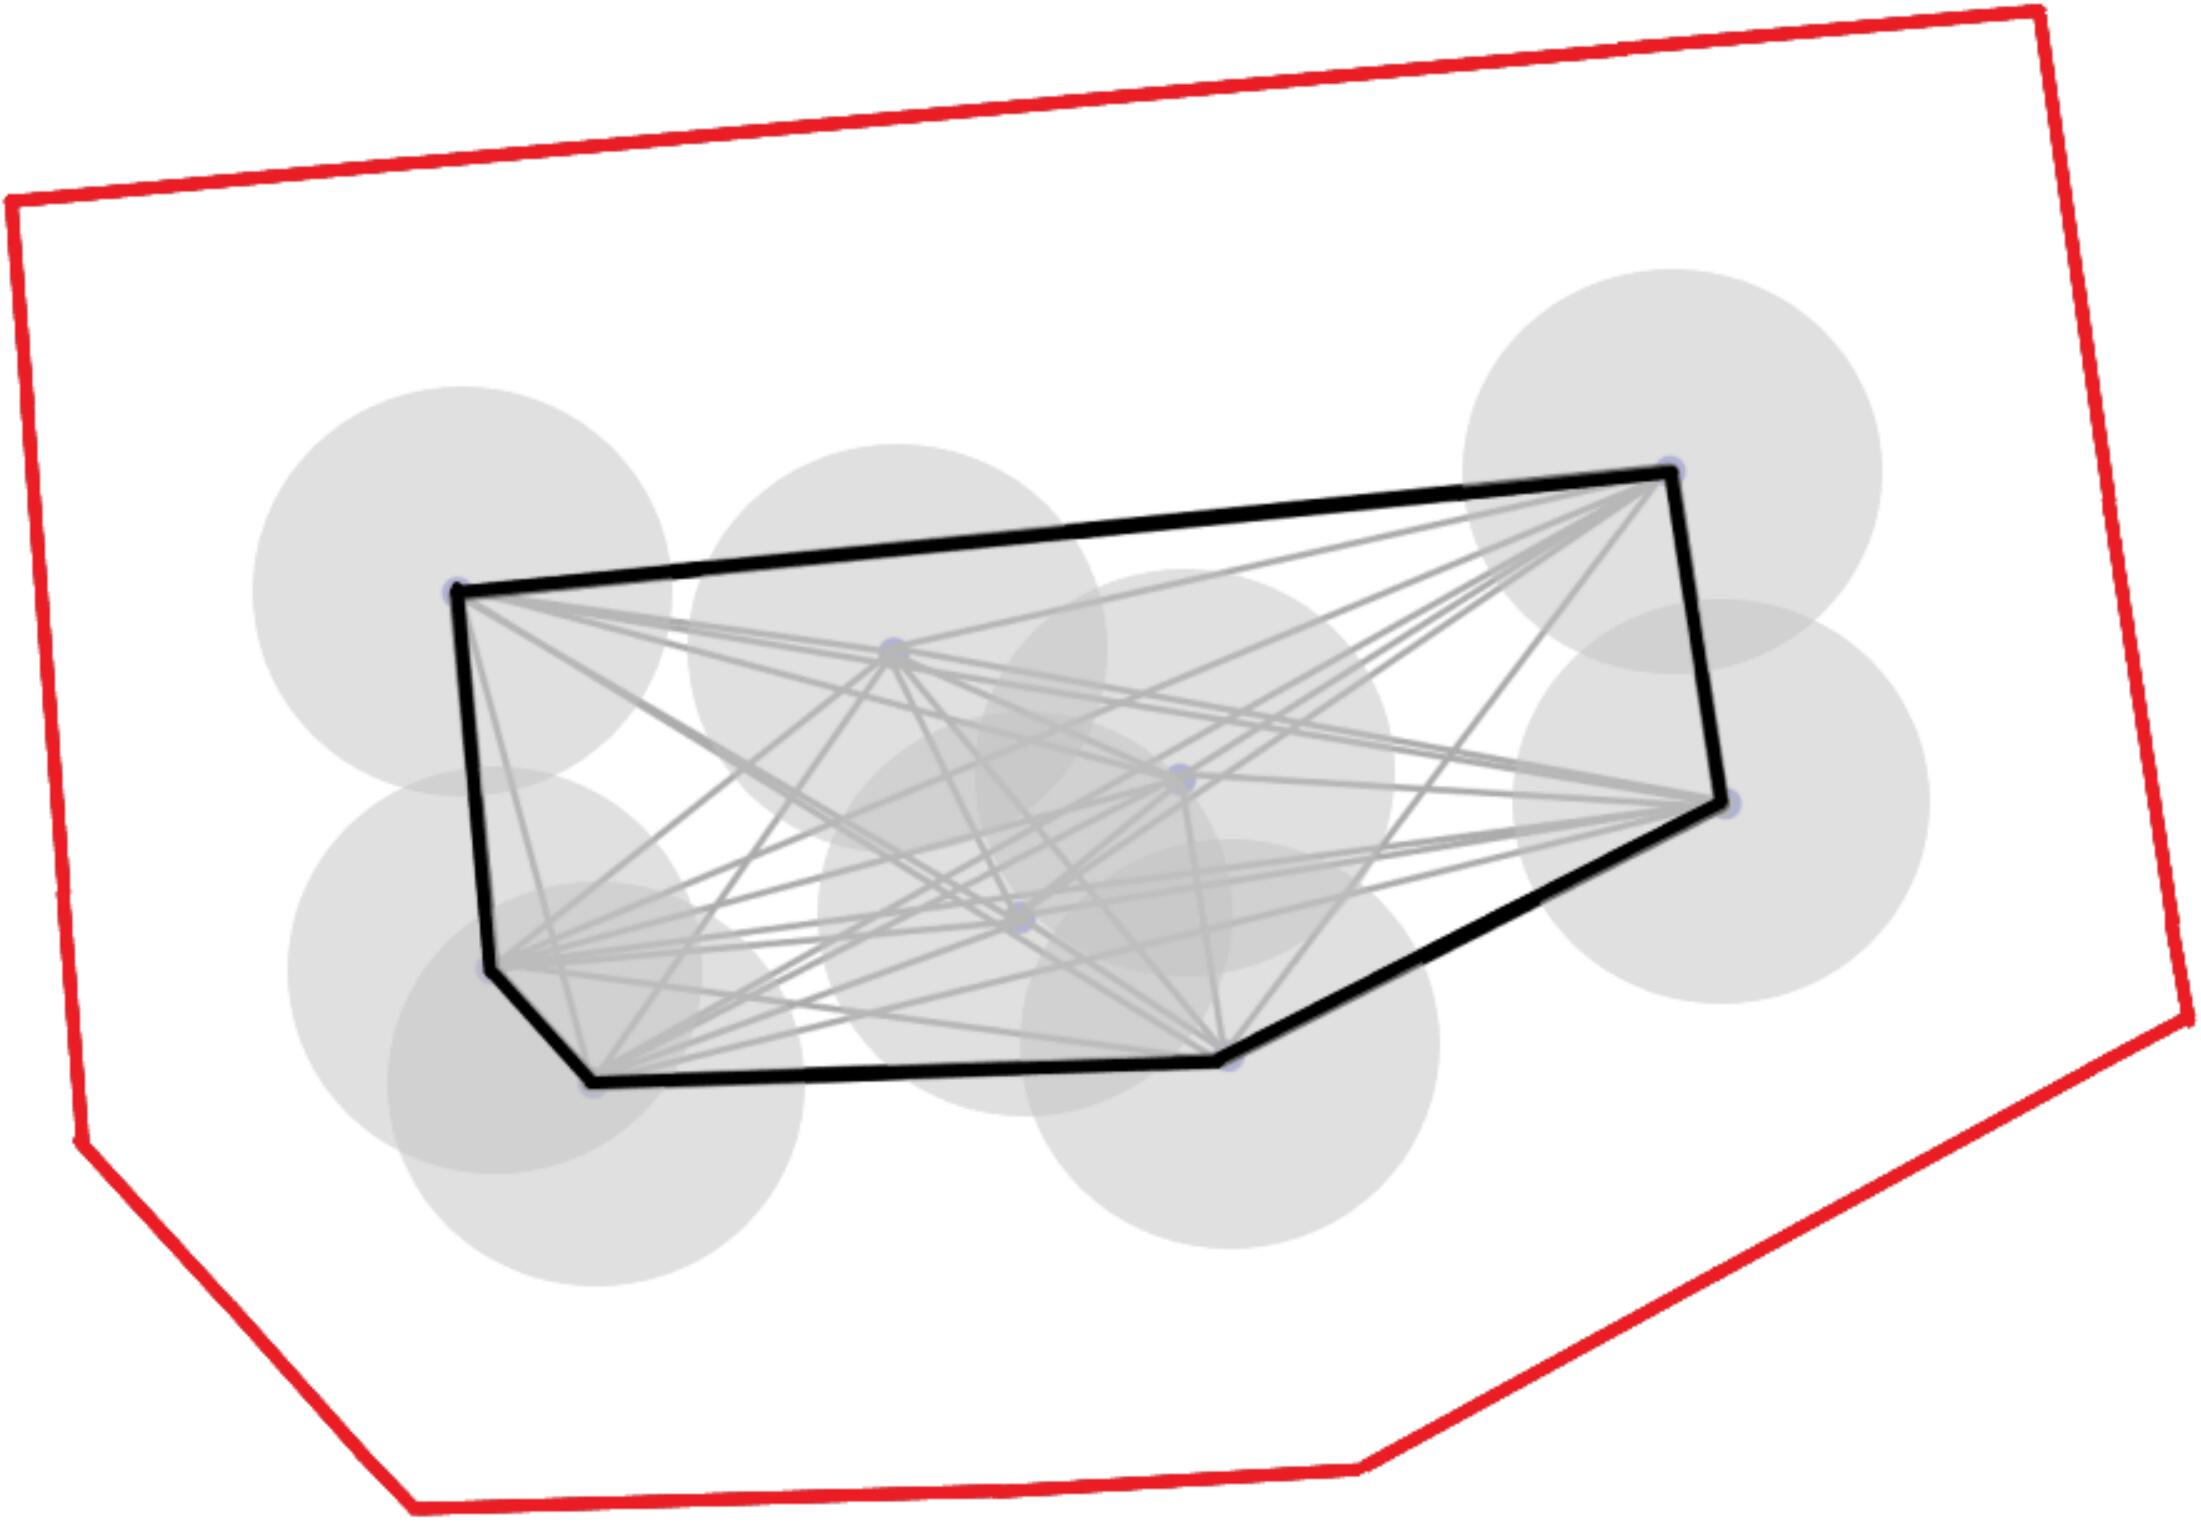
\includegraphics[width=9cm]{total_area.jpg}
	\caption{an example of the calculation of the total area}
	\label{fig:total_area}
\end{figure}

After going through an amount of residential and merchant areas, we can safely suppose that the distance from resident areas to the nearest merchant is within two times the radius of the coverage circle. The thin black lines connect each 2 merchants. The bold lines are the outermost lines and they form a polygon. Since the residential area usually appears to be like rectangles, we draw lines parallel with each side outside the polygon. These lines are connected to form the red line, which shows the total area border.

What we need to do is developing $RC=f(n)$. Obviously,
\[  \begin{cases}
f(0) = 0 \\
\frac{d}{dn} RC > 0 \\
0 \le RC < 1 \\
\frac{d}{d^2n} RC^2 < 0
\end{cases}  \]

Two common functions fit the requirements:
$ f(n) = \frac{n}{n+k} $ and $ f(n) = -k^n+1 $.
We search for some typical places where there are merchants among several residential areas. By \textit{Monte Carlo} method, we calculate several $(n,RC)$ and get the best $k$ and the best function through curve fitting.

\[f(n) = -k^n+1\]

Coefficients (with 95\% confidence bounds):
\[k = 0.8305  (0.8182, 0.8429)\]

\begin{center}
Goodness of fit:

  SSE: 0.002902
  
  R-square: 0.9912
  
  Adjusted R-square: 0.9912
  
  RMSE: 0.02409
\end{center}

\begin{figure}[H]
	\centering
	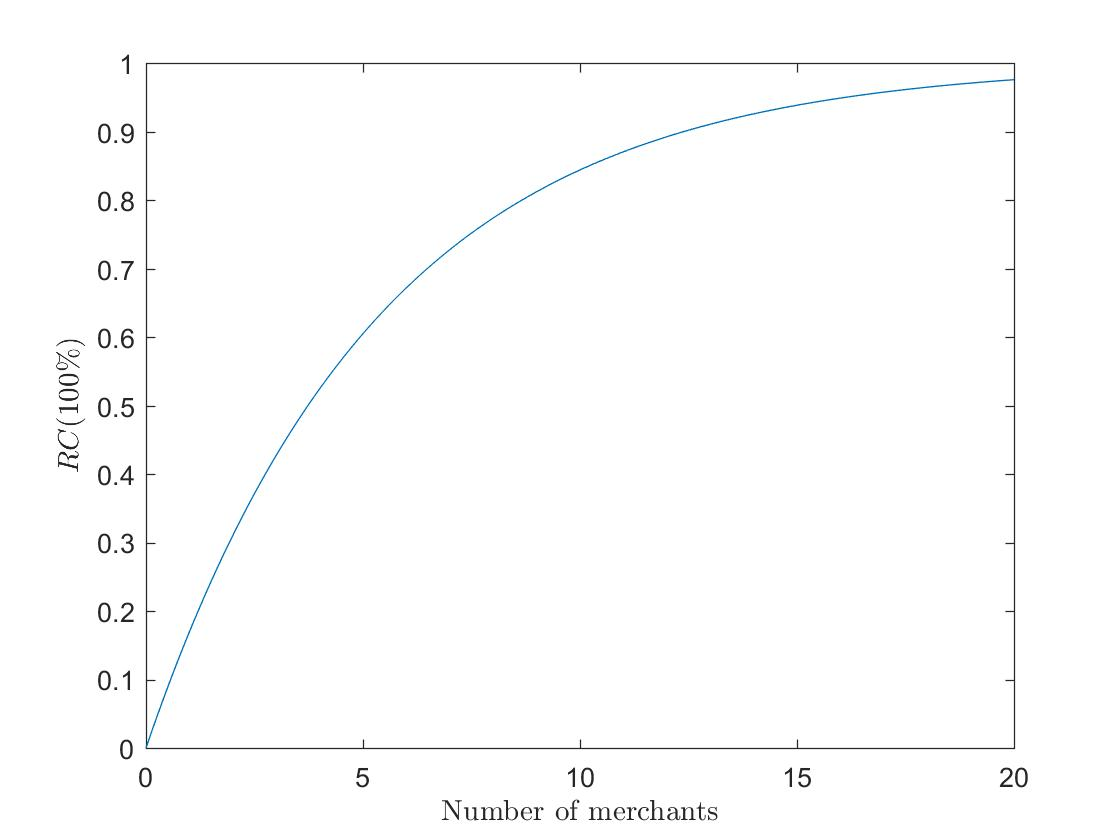
\includegraphics[width=10.5cm]{RC_function.jpg}
	\caption{the image of function RC=f(n)}
	\label{fig:RC_function}
\end{figure}

\subsubsection{Advertising Impact}
The $I_A$, as its name indicates, has a linear relationship with the times an ally is advertised. Hence, $I_A \propto (n-1)$. So we consider
\[  I_A = k_A (n-1)  \]
in which $k_A$ is a constant that will be measured later.

\subsubsection{Drowning Impact}
The $I_D$ is straightly related to the scale of the ally and the scale sum of all allies in the alliance.

The higher the reputation of an ally in the alliance, the less it will suffer from the \textsl{Drowning Effect}.

Suppose
\[  s = \frac{s_X}{\overline{s}} 
= \frac{n \cdot s_x}{\sum\limits_{i=1}^n S_i}  \]

So,
\[
I_D \propto
\frac{\textup{the total scale of the alliance}}{\textup{the relative scale of the ally}}
=
\frac{u(s_1,s_2,\ldots,s_n)}{v(s)}
\]

Obviously, the relationship between $s$ and $I_D$ is not linear. It should fit in with
\[\begin{cases}
\frac{d}{ds} I_D < 0 \\
\frac{d}{d^2s} {I_D}^2 > 0 \\
\forall i,j \in \{1,2,\ldots,n\}, S_i < S_j,
\frac{\partial u}{\partial S_i} < \frac{\partial u}{\partial S_j}
\end{cases}\]

By calculating with calculus, we find a suitable answer.
\[
u(s_1,s_2,\ldots,s_n) = \sum\limits_{i=1}^n {s_i}^2
\]

\[  v(s) = e^x  \]

So for the $I_D$, as is shown in figure \ref{fig:drowning_effect},
\[  I_D = \frac{\sum\limits_{i=1}^n {s_i}^2}{e^s}  \]
\begin{figure}[H]
\centering
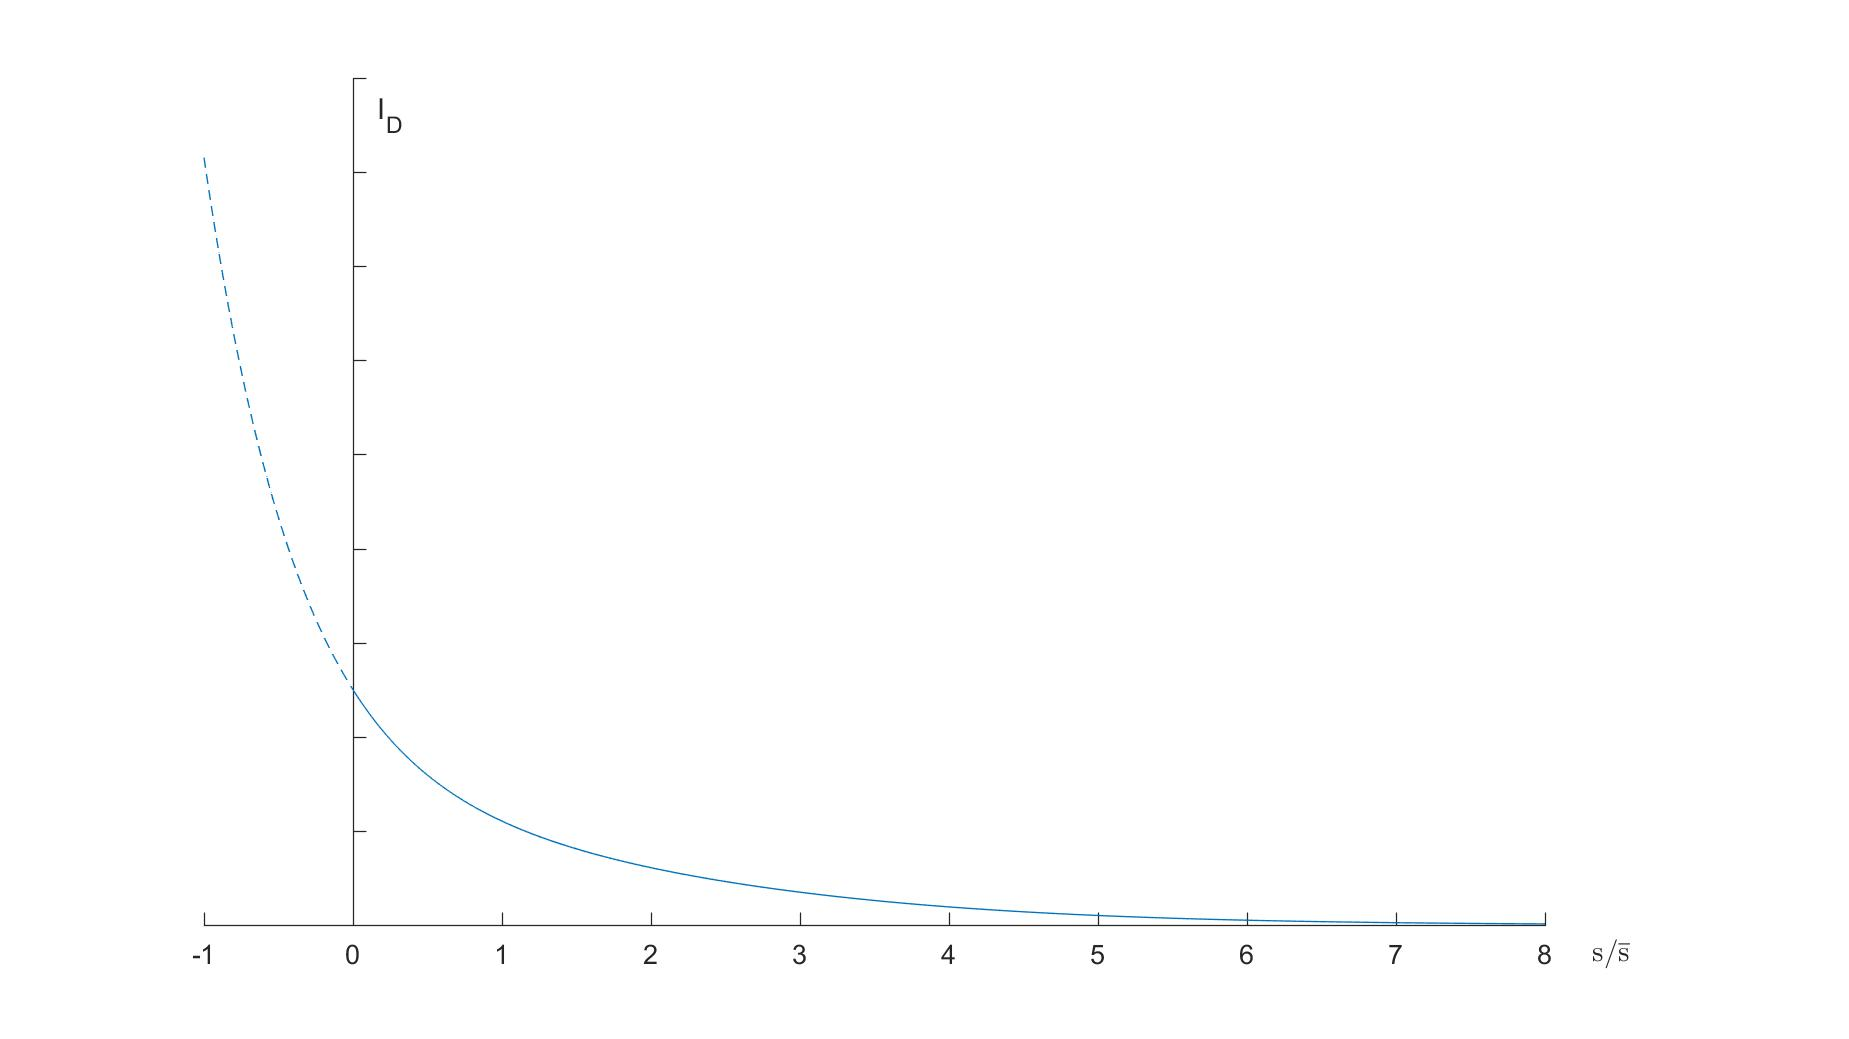
\includegraphics[width=0.7\linewidth]{drowning_effect.jpg}
\caption{the relationship between relative $I_D$ and scale of the ally}
\label{fig:drowning_effect}
\end{figure}

\begin{figure}[H]
\centering
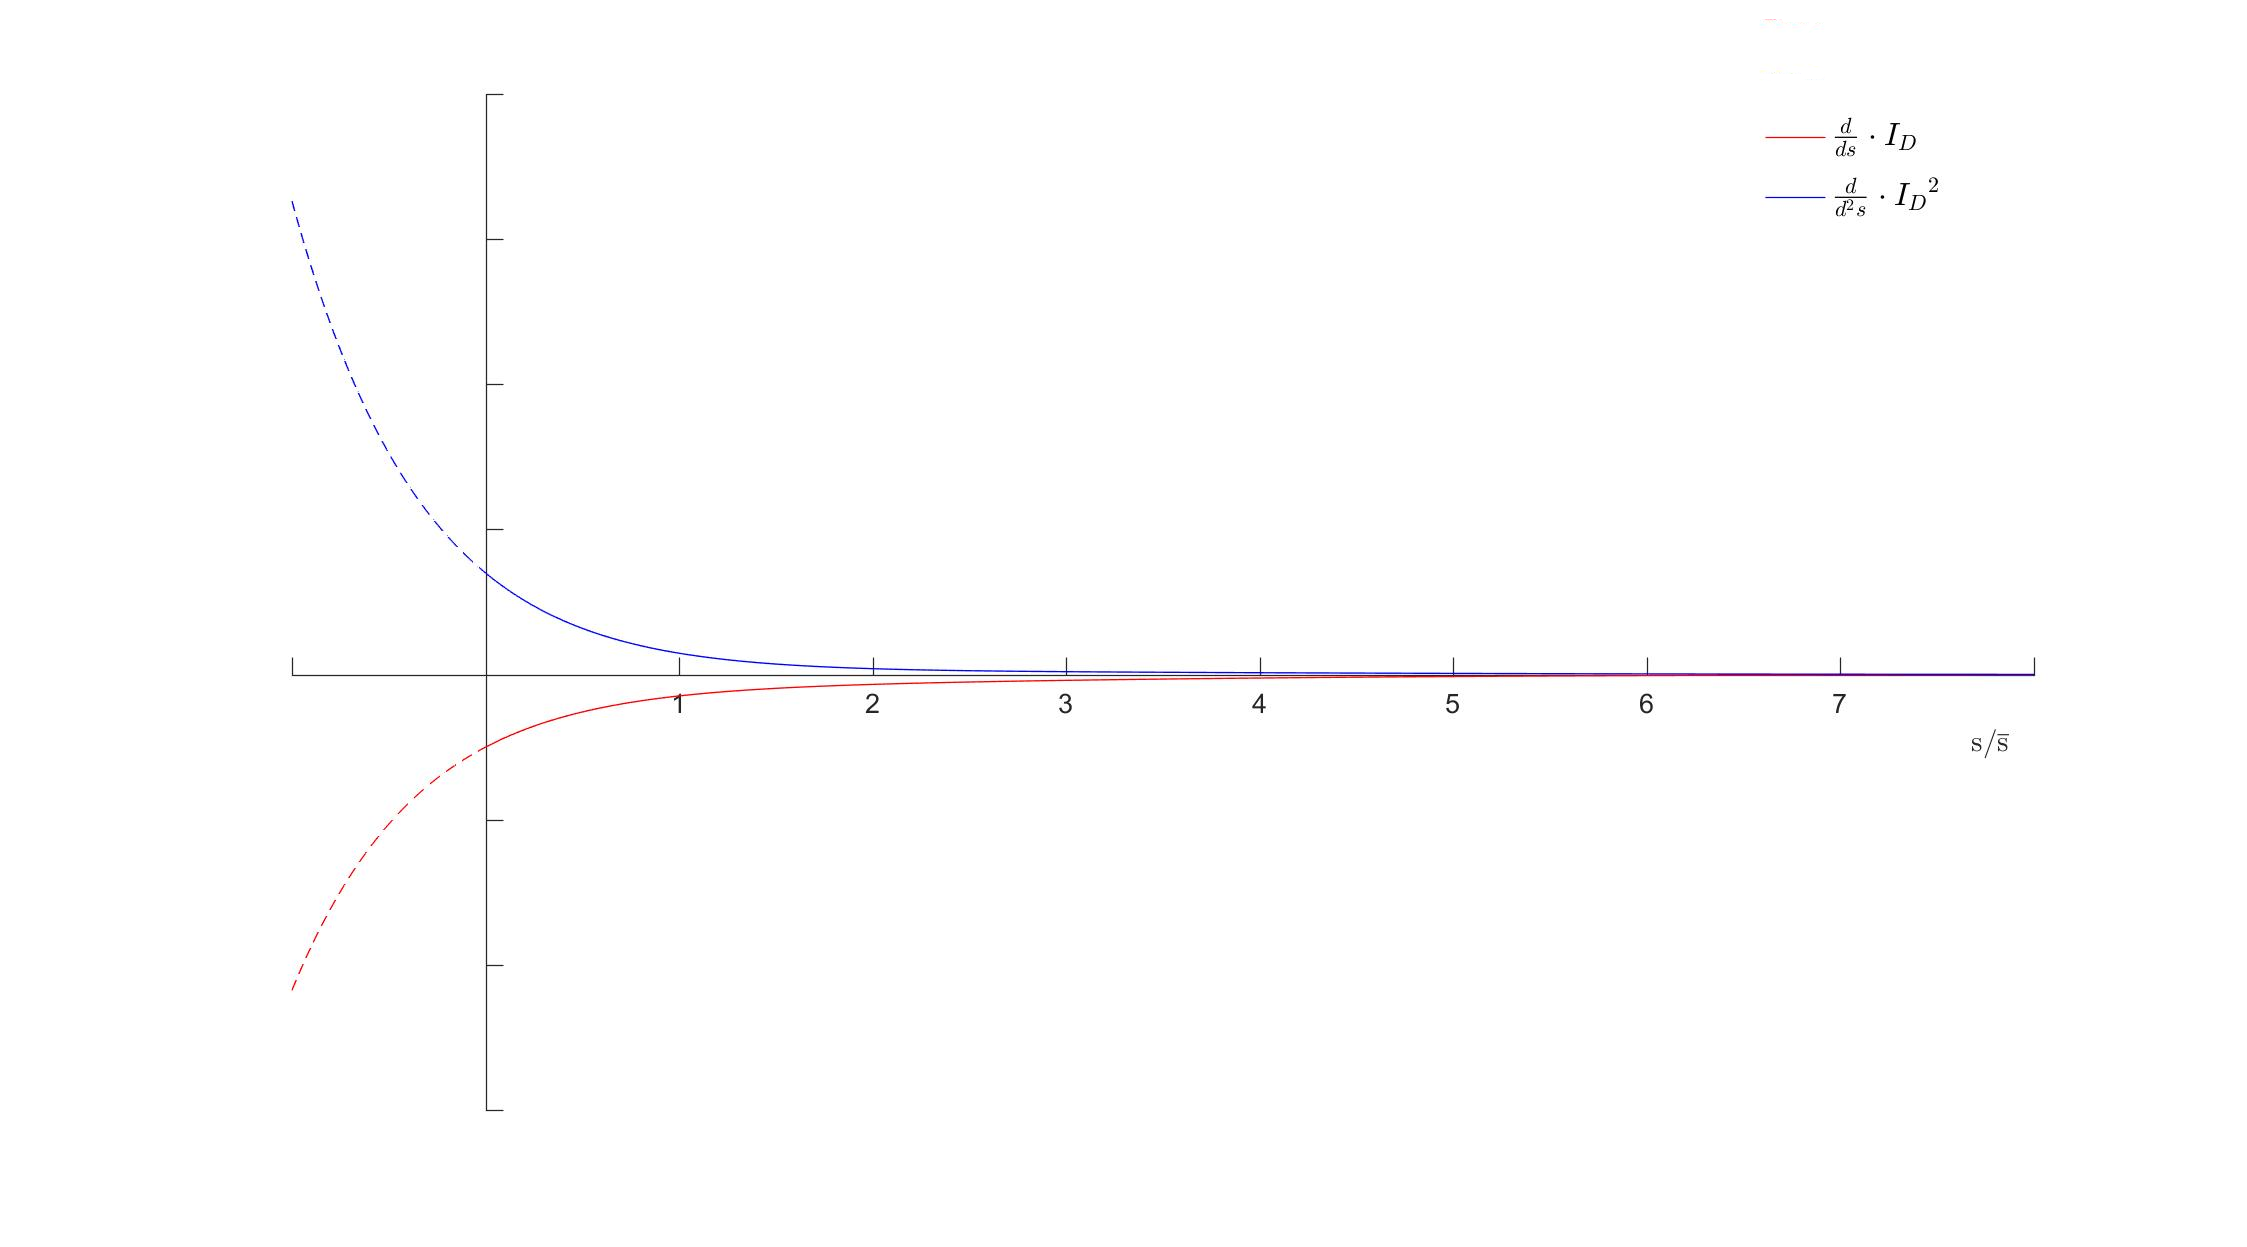
\includegraphics[width=0.7\linewidth]{drowning_effect_calculus.png}
\caption{the features of the relationship between relative $I_D$ and scale of the ally}
\label{fig:drowning_effect_calculus}
\end{figure}

\subsubsection{Product Type}
We decompose the overall impact of product type on \X{X}\ ($\Phi_X$) into several sub-impact for every product type.

Let us make our object the impact from product type of \B\ to \A. Then we calculate the overlapping rate of each column (universal product type classification).
\[  \phi_{i,B} = 
\frac{\sum_{\begin{subarray}{c}
\textup{for each overlapping} \\ \textup{Product}\ i
\end{subarray}} P_i}%
{\sum_{\begin{subarray}{c}
\textup{for each } \\ \textup{Product}\ j
\end{subarray}} P_j}  \]

\[  \phi_B = \sum\limits_{i=1}^{M_i} \phi_{i,B}  \]

Here is an example of the calculation of $\phi$. Its final result is $\Phi=171\%$.

\begin{table}[H]
\begin{tabular}{|c|p{.7\textwidth}|c|}
\hline
Product Type & Products & $\phi_{i,B}$ \\
\hline
Dishwasher & \tabincell{l}{(A) \$359.99, \$350.00 \\ (B) \$349.00, \$330.00 \\ (A\&B) \$512.80, \$399.99} & 39.7\% \\
\hline
Microwave Oven & \tabincell{l}{(A) \$99.98, \$212.40 \\ (B) \$59.98, \$95.30, \$111.99 \\ (A\&B) \$96.67, \$134.99} & 28.6\% \\
\hline
Refrigerator & \tabincell{l}{(A) \$783.19, \$511.40 \\ (B) \$599.00, \$872.02 \\ (A\&B) \$279.00, \$635.33} & 24.8\% \\
\hline
Laundry & \tabincell{l}{(A) \$205.99, \$279.99 \\ (B) \$163.99 \\ (A\&B) \$253.33, \$249.99, \$323.51} & 56.0\% \\
\hline
Range Hood & \tabincell{l}{(A) \$323.82, \$382.21 \\ (B) \$359.26, \$290.91, \$284.99 \\ (A\&B) \$459.96} & 21.9\% \\
\hline
\end{tabular}
\caption{an example of the calculation of $\phi$}
\label{tab:phi_calc}
\end{table}

Now the last problem is how to sum up the impact of each ally to the merchant. By market experience, one suitable relationship between $\phi_X$ and $\Phi_{X}$ is
\[  \Phi_{X} = {\sum_{X=1}^{n-1} \phi_X}  \]
\[  = {\sum_{X=1}^{n-1} {\sum\limits_{i=1}^{M_i} \phi_{i,X}}}  \]

\subsubsection{Overall Algorithm}
For a certain ally,
\[  I = \Phi \cdot RC \cdot (I_A - I_D)  \]
\[  = {\sum_{X=1}^{n-1} \phi_X} \cdot (-0.8305^n+1) \cdot \left[k_A (n-1) - \frac{\sum_{i=1}^n {s_i}^2}{e^s}\right]   \]
\[  = {\sum_{X=1}^{n-1} {\sum\limits_{i=1}^{M_i} \phi_{i,X}}} \cdot (-0.8305^n+1) \cdot \left[k_A (n-1) - \frac{\sum_{i=1}^n {s_i}^2}{e^s}\right]  \]

The relative importance will be further discussed in the section \textsl{Sensitivity Analysis}.

Then we test the model result. We get the value of the constant $k_A=50$ and make a modification to modify $I$'s order of magnitude. The final result is
\begin{equation}
I = \left({\sum_{X=1}^{n-1} {\sum_{i=1}^{M_i} \phi_{i,X}}} \cdot (-0.8305^n+1) \cdot \left[50(n-1) - \frac{\sum_{i=1}^n {s_i}^2}{e^{\sqrt{s}}}\right]\right)^\frac{1}{3}
\label{eq:mtm_model}
\end{equation}

	\subsection{Sensitivity Analysis}
	To assess the robustness of our model, we conduct sensitivity analyses on several arguments ($n$,$s$,$\phi$) in Equation \ref{eq:mtm_model}.

\begin{enumerate}
\itembf{the number of merchants ($n$)}

\begin{figure}[H]
\centering
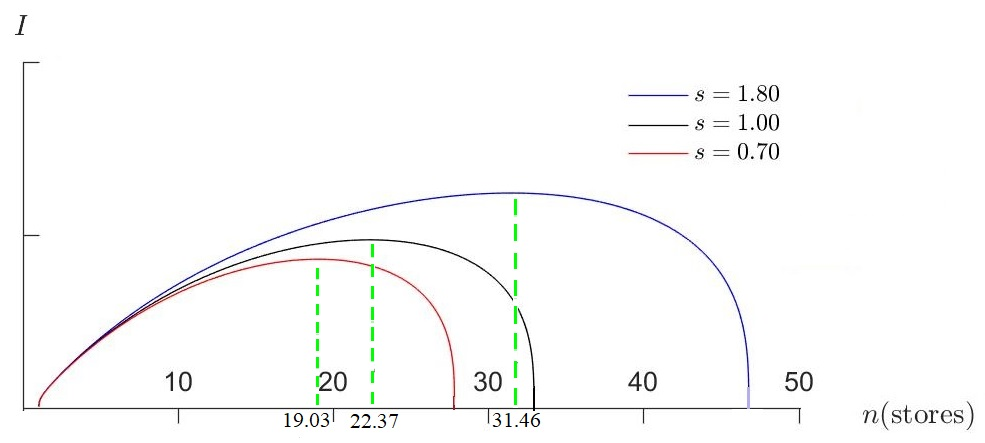
\includegraphics[width=9cm]{sa_mtm_n.jpg}
\caption{the sensitivity of $n$ on $I$}
\label{fig:sa_mtm_n}
\end{figure}

Figure \ref{fig:sa_mtm_n} shows the relationship between $n$ and $I$ under three certain $s$. Obviously $I_{\max}$ is directly related to $n$ under the same $s$, thus proving that our model is effective.

The figure also serves as a virtual show of our model result. The scale will affect $I_{\max}$. It also reveals a truth that the optimal $n$ for each ally varies.

\itembf{the relative scale of the object merchant}

\begin{figure}[H]
\centering
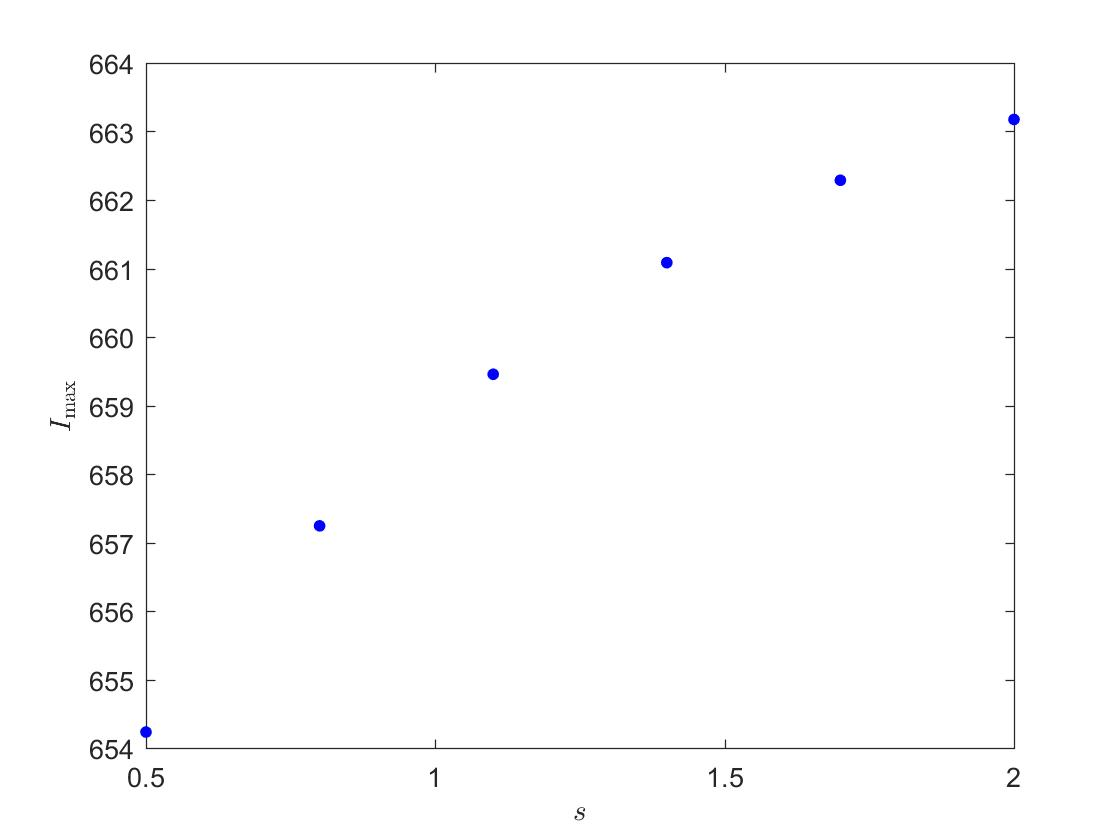
\includegraphics[width=9cm]{sa_mtm_s.jpg}
\caption{the sensitivity of $s$ on $I$}
\label{fig:sa_mtm_s}
\end{figure}

As Figure \ref{fig:sa_mtm_s}\ shows, our model is not sensitive to the relative scale of the object merchant $s$. This indicates that under the same $n$, the business status of the object merchant will not affect its bonus profit, proving that our model is quite robust. And it is worth mentioning that the $n$ in this part of the analysis may not be the optimal $n$ for the object merchant. In fact, it at most time actually isn't.

%\itembf{the overlapping index of all allies to the object merchant}

%\begin{figure}
%\centering
%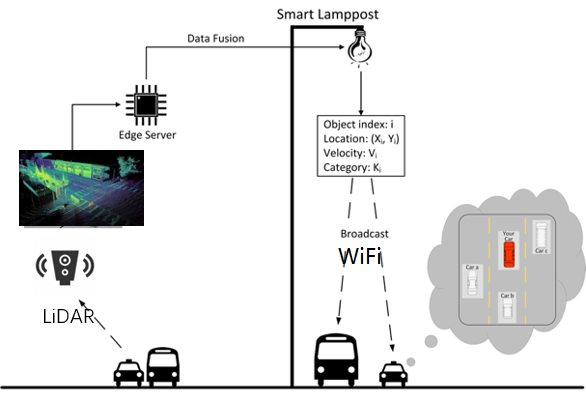
\includegraphics[width=9cm]{mechanism.png}
%\caption{the sensitivity of $\phi$ on $I$}
%\label{fig:sa_mtm_phi}
%\end{figure}

\itembf{the average scale of all allies (\textnormal{the solution to } 2(c))}

\begin{figure}[H]
\centering
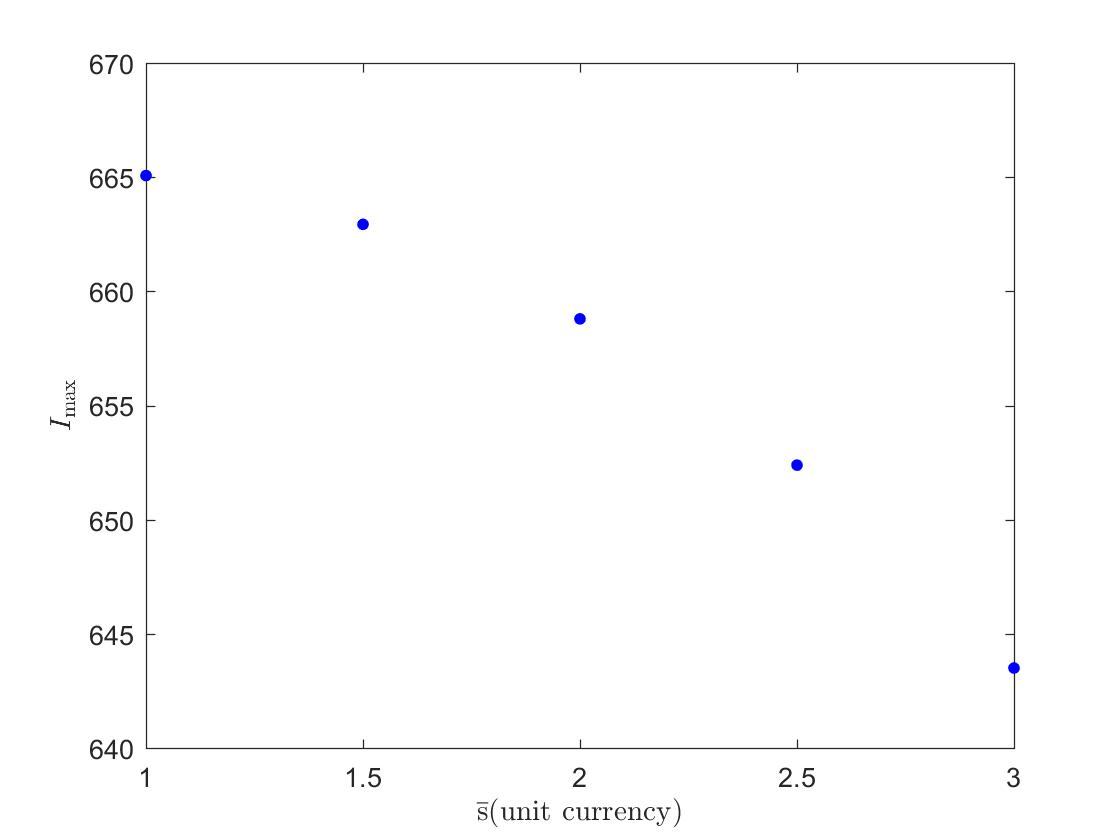
\includegraphics[width=9cm]{sa_mtm_osi.jpg}
\caption{the sensitivity of an $s_i$ on $I$}
\label{fig:sa_mtm_osi}
\end{figure}

In equation \ref{eq:mtm_model}, for the object merchant, $s_1,s_2,\ldots,s_{n-1}$ all serve as constants. So in this part of the sensitivity analysis, we conduct the analysis on one constant $\overline{s_i}$.

The result is that $I$ is not sensitive to $s_i$, meaning that the scale of the allies does not make a difference to the ideal alliance mode. So the change in yearly revenue of allies will not affect our model.

\itembf{the number of Product Type in the universal classification}

\begin{figure}[H]
\centering
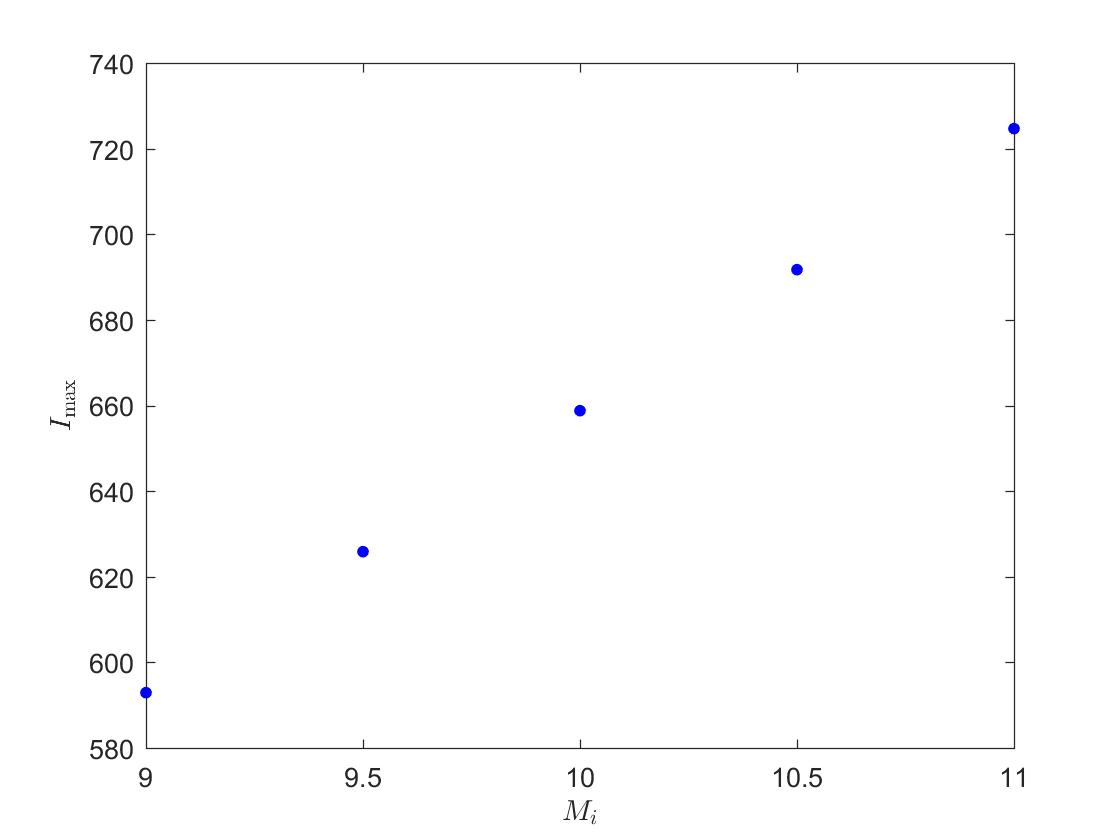
\includegraphics[width=9cm]{sa_mtm_mi.jpg}
\caption{the sensitivity of an $M_i$ on $I$}
\label{fig:sa_mtm_mi}
\end{figure}

Since $M_i$ indicated the resolution of the product type classification, its size should only affect the accuracy of the $I_{\max}$. However, our model is relatively quite sensitive to $M_i$, making it fragile.
\end{enumerate}
	
	\section{Reward Points Distribution}
	\subsection{Model Assumptions}
	\begin{enumerate}
\item
The higher the market value of an ally, the more weight its word carries, and thus the higher its benefit.

\textsl{This assumption is based on experience from all fields, and successfully decides the balanced $I$ in the alliance.}
\end{enumerate}
	\subsection{General Route}
	From Figure \ref{fig:sa_mtm_n}\ we can know that the optimal $n$ for each ally is not the same. And the \textsl{Model Assumption 1}\ can be described as
\begin{equation}
\epsilon = \frac{RP}{\sqrt{\theta}} + g(\Phi) \to c\ \textup{(for each ally)}
\label{eq:I_theta_relationship}
\end{equation}
in which $c$ is a constant whose value does not matter.
	\subsection{Solution}
	From Equation \ref{eq:I_theta_relationship}\ we can know that at the balance status of the alliance, all $\epsilon$\ should be as close as possible, describing as
\[  \sigma^{2} = \frac{\sum_{i=1}^{n}(\epsilon_i-\mu)^{2}}{n} \to 0  \]
in which $\mu$ is the average $\epsilon$.

The final result shows that $\epsilon$ is actually not sensitive with $\Phi$. So the relationship turns out to be
\[  RP = c \cdot \sqrt{\theta}  \]
So the optimal distribution should simply be
\[  RP_1 : RP_2 : \ldots : RP_n = \sqrt{\theta_1} : \sqrt{\theta_2} : \ldots : \sqrt{\theta_n}  \]
	
	\section{Strengths and Weaknesses}
	\subsection{Strengths}
\begin{enumerate}
\itembf{Our one-to-one model is independent of external data.}

The model is solely dependent on products and purchases data, which can be directly obtained from the merchants. Therefore, our model is quite robust, so it can be applied to any one-to-one alliances.

\itembf{Our one-to-one model is data efficient.}

The model calculates the profit growth, which is relatively stable in all time of a year. Therefore, we can estimate the year's profit growth by collecting data for a short period of time.

\itembf{Our many-to-many model is highly efficient.}

The algorithm only requires the market values, and product type and price from each ally, plus the total number of allies, which is easy to obtain. Therefore, our many-to-many model does not need much data to give the estimation result.

\itembf{Our many-to-many model is robust.}

All arguments in the algorithm are product information and the scale of the allies, which can not be changed overnight. This makes our estimation model robust. Additionally, the many-to-many model is not based on many assumptions, making it not at all fragile, and in other words, robust.
\end{enumerate}

\subsection{Weaknesses}
\begin{enumerate}
\itembf{Our many-to-many model is based on assumptions.}

For example, we assumed that the cover range of each merchant is a circle with a radius of 0.2km. The radius actually varies in real life. The assumptions make our model fragile.

\itembf{Datasets are lacked to precisely decide the value of the constants in our many-to-many model.}

Our functions are based on experience of the marketplace and logic. But only with enough datasets can the constants be accurately measured and decided. Our lack of dataset sources makes the estimate result not relatively accurate.

\itembf{Our m-m model is to some extent sensitive.}

By sensitivity analysis, we get to know that our model is somehow sensitive to $M_i$, which means that the resolution of the product type classification will affect the $I_{\max}$, making our model fragile.

\itembf{Our model neglects the impact brought about by the correlation of products between each two allies.}

The existence of product correlation can bring extra benefit to merchants since they will have an overlapping customer group. However, it's hard to quantify and calculate. So we neglect its impact, and thus lower our model effect.
\end{enumerate}
	
	\pagebreak
	\appendix
	\section{One-to-One Alliance Revenue Estimation Algorithm}
	\subsection{Source Code}
	\begin{lstlisting}[language=C++]
#include<bits/stdc++.h>
#include<fstream>
#include<sstream>
#define M1 5
#define M2 6
#define M3 4 
#define C 100000 
#define PT 1000
#define P 100000
#define S 2
using namespace std;
int typ,old_purc[M1],purc[M2],prd[P][M3],yes_sell[S][P],label[C];//label 1:OnlyA 2:OnlyB 3:A&B 
double old_time,now_time,freq[C][S][PT],total_freq[S][PT],total_total_freq[S],rp_used[S][PT],rp_loss[S][PT],total_rp_loss[S],k1,k2;
char typ_name[PT];
void up_pctg(double a,double b){
	double rate=a/b*100;
	cout<<rate<<"%"<<endl;
}
int main(){
	cout<<"How many types of goods:";
	cin>>typ;
	cout<<"Please input the symbols of the "<<typ<<" types of goods."<<endl;
//	for(int i=0;i<typ;i++)cin>>typ_name[i];
	cout<<"Please input the rate from(to) money to(from) RPs:";
	cin>>k1>>k2;
	
	
	
	int overlap[P]={0};//1A2B3AB
	double overlap_cnt=0,t=0;
	string line;
	ifstream fin("prd.csv");
	while(getline(fin,line)){
		istringstream sin(line);
		vector<string> data;
		string info;
		while(getline(sin,info,',')){
			data.push_back(info);
			if(info=="\n")break;
		}
		int tt=int(t);
		for(int i=0;i<M3;i++)prd[tt][i]=atoi(data[i].c_str());//id price typ_id shop(0A1B)
		
		yes_sell[prd[tt][3]][prd[tt][2]]=1;
		
		if(prd[tt][3]==0&&overlap[tt]==2)overlap[tt]=2;
		if(prd[tt][3]==1&&overlap[tt]==1)overlap[tt]=2;
		if(overlap[tt]==0)overlap[tt]=prd[tt][3]+1;
		
		t++;
	}
	for(int i=0;i<t;i++)
		if(overlap[i]==3)overlap_cnt++;
	double overlap_rate=overlap_cnt/t;
	fin.close();
	
	
	
	cout<<"Please input the time span of the old data:";
	cin>>old_time;
	ifstream finn("old.csv");
	while(getline(finn,line)){
		istringstream sin(line);
		vector<string> data;
		string info;
		while(getline(sin,info,',')){
			data.push_back(info);
			if(info=="\n")break;
		}
		for(int i=0;i<M1;i++)old_purc[i]=atoi(data[i].c_str());//id customer_id product_id amount shop(0A1B)
		
		freq[old_purc[1]][old_purc[4]][prd[old_purc[2]][2]]+=prd[old_purc[2]][1]*old_purc[3];//by customer&shop&product type
		total_freq[old_purc[4]][prd[old_purc[2]][2]]+=prd[old_purc[2]][1]*old_purc[3];
		total_total_freq[old_purc[4]]+=prd[old_purc[2]][1]*old_purc[3];
		
		if(old_purc[4]==0){
			if(label[old_purc[1]]==2||label[old_purc[1]]==3)label[old_purc[1]]==3;
			else label[old_purc[1]]==1;
		}
		if(old_purc[4]==1){
			if(label[old_purc[1]]==1||label[old_purc[1]]==3)label[old_purc[1]]==3;
			else label[old_purc[1]]==2;
		}
	}
	for(int i=0;i<C;i++){
		for(int j=0;j<PT;j++){
			freq[i][0][j]/=old_time;
			freq[i][1][j]/=old_time; 
		}
	}
	for(int i=0;i<PT;i++){
		total_freq[0][i]/=old_time;
		total_freq[1][i]/=old_time;
	}
	total_total_freq[0]/=old_time;
	total_total_freq[1]/=old_time;
	finn.close();
	
	
	
	cout<<"Please input the time span of the new data:";
	cin>>now_time;
	double sales[2]={0};
	double total_rp_used[2]={0},total_total_rp_used=0,total_sales=0;
	double bonus_A[PT]={0},bonus_B[PT]={0};//by product type
	double total_bonus_A=0,total_bonus_B=0;
	ifstream finnn("now.csv");
	while(getline(finnn,line)){
		istringstream sin(line);
		vector<string> data;
		string info;
		while(getline(sin,info,',')){
			data.push_back(info);
			if(info=="\n")break;
		}
		for(int i=0;i<M2;i++)purc[i]=atoi(data[i].c_str());//id customer_id product_id amount use_rp shop(0A1B)
		rp_used[purc[5]][prd[purc[2]][2]]+=purc[4];
		total_rp_used[purc[5]]+=purc[4];
		total_total_rp_used+=purc[4];
		sales[purc[5]]+=prd[purc[2]][1]*purc[3];
		total_sales+=sales[purc[5]];
		
		if(purc[5]==1){
			bonus_B[prd[purc[2]][2]]+=purc[3]*prd[purc[2]][1];
			total_bonus_B+=purc[3]*prd[purc[2]][1];
		}
		if(purc[5]==0){
			bonus_A[prd[purc[2]][2]]+=purc[3]*prd[purc[2]][1];
			total_bonus_A+=purc[3]*prd[purc[2]][1];
		}
	}
	for(int i=0;i<PT;i++){
		rp_loss[0][i]=rp_used[1][i]*k2;
		rp_loss[1][i]=rp_used[0][i]*k2;
	}
	total_rp_loss[0]+=total_rp_used[1]*k2;
	total_rp_loss[1]+=total_rp_used[0]*k2;
	double rp_given[2]={sales[0]*k1,sales[1]*k1};
	double rp_rate[2]={total_rp_used[1]/rp_given[0],total_rp_used[0]/rp_given[1]};
	double total_rp_given=total_sales*k1;
	double total_rp_rate=total_total_rp_used/total_rp_given;
	for(int i=0;i<C;i++){
		if(label[i]==3){
			total_bonus_A-=now_time*total_freq[0][i];
			total_bonus_B-=now_time*total_freq[1][i];
		}
	}
	finnn.close();
	
	
	
	cout<<"==============="<<endl;
	cout<<"Money to RP: "<<k1<<endl;
	cout<<"RP to Money: "<<k2<<endl;
	cout<<"The total RP usage rate: "<<total_rp_rate<<endl;
	cout<<"Overlap Rate: "<<overlap_rate<<endl; 
	cout<<"Merchant A benefit rise: ";
	up_pctg(total_bonus_A-total_rp_loss[0],now_time*total_total_freq[0]);
	cout<<"With each kind of product rising: "<<endl;
	for(int i=0;i<typ;i++){
		if(!yes_sell[0][i])continue;
		cout<<typ_name[i]<<": ";
		up_pctg(bonus_A[i]-rp_loss[0][i],now_time*total_freq[0][i]);
	}
	cout<<"Merchant B benefit rise: ";
	up_pctg(total_bonus_B-total_rp_loss[1],now_time*total_total_freq[1]);
	cout<<"With each kind of product rising: "<<endl;
	for(int i=0;i<typ;i++){
		if(!yes_sell[1][i])continue;
		cout<<typ_name[i]<<": ";
		up_pctg(bonus_B[i]-rp_loss[1][i],now_time*total_freq[1][i]);
	}
	cout<<"==============="<<endl;
	return 0;
}
\end{lstlisting}

	\subsection{User Guide}
	\sffamily
\textbf{\large Files}

\begin{enumerate}
\itemsl{old.csv}

Stores the records of purchases before the alliance formed. 5 params are "id", "customer\_id", "product\_id", "amount", "shop". For param "shop", 0 stands for Shop A while 1 stands for B.

\itemsl{new.csv}

Stores the records of purchases after joining the alliance. 6 params are "id", "customer\_id", "product\_id", "amount", "rp\_usage", "shop". For param "shop", 0 stands for Shop A while 1 stands for B.

\itemsl{prd.csv}

Stores the information of products in both shops. 4 params are "id", "price", "type\_id", "shop". For param "shop", 0 stands for Shop A while 1 stands for shop B. Data in param "type\_id" should start from 0.
\end{enumerate}

Please note that the code has a high requirement for your input accuracy. The file shall not contain extra spaces or letters.
\newline \newline
The three files should be placed in the same folder or under the same path as the .exe file.
\newline \newline
After you are prepared, double-click on the .exe file.
\newline \newline
\textbf{\large Inputs}
\newline \newline
Please follow the prompt and input all the data required. Inputs shall not contain extra spaces or letters. Press Enter after typing in the numbers and wait for the next prompt.
\newline \newline
\textbf{\large Demo}
\begin{lstlisting}[basicstyle=\sffamily]
The output should look like this:

===============
Money to RP: 0.1
RP to Money: 0.1
The  total RP usage rate: 0.25
Overlap Rate: 0.3333333
Merchant A benefit rise: 9.2135743%
With each kind of product rising:
a: 3.1428965%
b: 8.1263814%
c: 12.2183681%
Merchant B benefit rise: 7.2368624%
With each kind of product rising:
b: 6.2438914%
c: 7.4683649%
d: 8.2343749%
===============

If you run into any problems, feel free to contact the support group. 
\end{lstlisting}
(\textit{example@example.com})
\rmfamily
\end{document}